\documentclass[11pt,twocolumn,oneside,openany,headings=optiontotoc,11pt,numbers=noenddot]{article}

\usepackage[a4paper]{geometry}
\usepackage[utf8]{inputenc}
\usepackage[T1]{fontenc}
\usepackage{lmodern}
\usepackage[ngerman]{babel}
\usepackage{ngerman}

\usepackage[onehalfspacing]{setspace}

\usepackage{fancyhdr}
\usepackage{fancybox}

\usepackage{rotating}
\usepackage{varwidth}

%Struktogramme
\usepackage[german,curves]{struktex}

\usepackage{pdflscape}
\usepackage{changepage}
\usepackage{graphicx}
\usepackage[bottom]{footmisc}
\usepackage{transparent}
\usepackage{graphbox}
\graphicspath{
	{Pics/PDFs/}
	{Pics/JPGs/}
	{Pics/PNGs/}
}
\usepackage{caption}
\usepackage{wrapfig}
\usepackage{marginnote}
\usepackage{tabularx}
\usepackage{dashrule}
\usepackage{soulutf8}
\usepackage{hhline}
%arydshln suppresses vertical lines in table
%\usepackage{arydshln}
\usepackage{multirow}
\usepackage{enumerate}
\usepackage[hidelinks]{hyperref}
\usepackage{listings}

\usepackage[table]{xcolor}
\usepackage{array}
\usepackage{enumitem,amssymb,amsmath}
\usepackage{interval}
\usepackage{cancel}
\usepackage{stmaryrd}
\usepackage{wasysym}
\usepackage{polynom}
\usepackage{diagbox}
\usepackage{dashrule}
\usepackage{framed}
\usepackage{mdframed}
\usepackage{karnaugh-map}
\usepackage{pdfpages}

\usepackage{blindtext}

\usepackage{eso-pic}

\usepackage{amssymb}
\usepackage{eurosym}

\usepackage[pages=some]{background}
\pagestyle{headings}
\renewcommand{\headrulewidth}{0.2pt}
\renewcommand{\footrulewidth}{0.2pt}
\newcommand*{\underdownarrow}[2]{\ensuremath{\underset{\overset{\Big\downarrow}{#2}}{#1}}}
\setlength{\fboxsep}{5pt}
\newcommand{\explainBelow}[3]{\underbrace{#1}_{\parbox{\widthof{#3}}{\footnotesize\raggedright #2}}}
\newcommand{\explainAbove}[3]{\overbrace{#1}^{\parbox{\widthof{#3}}{\footnotesize\raggedright #2}}}
\newcommand\footnoteref[1]{\protected@xdef\@thefnmark{\ref{#1}}\@footnotemark}


% Codestyle defined
\definecolor{codegreen}{rgb}{0,0.6,0}
\definecolor{codegray}{rgb}{0.5,0.5,0.5}
\definecolor{codepurple}{rgb}{0.58,0,0.82}
\definecolor{backcolour}{rgb}{0.95,0.95,0.92}
\definecolor{deepgreen}{rgb}{0,0.5,0}
\definecolor{darkblue}{rgb}{0,0,0.65}
\definecolor{mauve}{rgb}{0.40, 0.19,0.28}
\colorlet{exceptioncolour}{yellow!50!red}
\colorlet{commandcolour}{blue!60!black}
\colorlet{numpycolour}{blue!60!green}
\colorlet{specmethodcolour}{violet}

%Neue Spaltendefinition
\newcolumntype{L}[1]{>{\raggedright\let\newline\\\arraybackslash\hspace{0pt}}m{#1}}
\newcolumntype{M}{>{\centering\arraybackslash}X}
\newcommand{\cmnt}[1]{\ignorespaces}
%Textausrichtung ändern
\newcommand\tabrotate[1]{\rotatebox{90}{\raggedright#1\hspace{\tabcolsep}}}

%Intervall-Konfig
\intervalconfig {
	soft open fences
}

%Bash
\lstdefinestyle{BashInputStyle}{
	language=bash,
	basicstyle=\small\sffamily,
	backgroundcolor=\color{backcolour},
	columns=fullflexible,
	backgroundcolor=\color{backcolour},
	breaklines=true,
}
%Java
\lstdefinestyle{JavaInputStyle}{
	language=Java,
	backgroundcolor=\color{backcolour},
	aboveskip=1mm,
	belowskip=1mm,
	showstringspaces=false,
	columns=flexible,
	basicstyle={\footnotesize\ttfamily},
	numberstyle={\tiny},
	numbers=none,
	keywordstyle=\color{purple},,
	commentstyle=\color{deepgreen},
	stringstyle=\color{blue},
	emph={out},
	emphstyle=\color{darkblue},
	emph={[2]rand},
	emphstyle=[2]\color{specmethodcolour},
	breaklines=true,
	breakatwhitespace=true,
	tabsize=2,
}
%Python
\lstdefinestyle{PythonInputStyle}{
	language=Python,
	alsoletter={1234567890},
	aboveskip=1ex,
	basicstyle=\footnotesize,
	breaklines=true,
	breakatwhitespace= true,
	backgroundcolor=\color{backcolour},
	commentstyle=\color{red},
	otherkeywords={\ , \}, \{, \&,\|},
	emph={and,break,class,continue,def,yield,del,elif,else,%
		except,exec,finally,for,from,global,if,import,in,%
		lambda,not,or,pass,print,raise,return,try,while,assert},
	emphstyle=\color{exceptioncolour},
	emph={[2]True,False,None,min},
	emphstyle=[2]\color{specmethodcolour},
	emph={[3]object,type,isinstance,copy,deepcopy,zip,enumerate,reversed,list,len,dict,tuple,xrange,append,execfile,real,imag,reduce,str,repr},
	emphstyle=[3]\color{commandcolour},
	emph={[4]ode, fsolve, sqrt, exp, sin, cos, arccos, pi,  array, norm, solve, dot, arange, , isscalar, max, sum, flatten, shape, reshape, find, any, all, abs, plot, linspace, legend, quad, polyval,polyfit, hstack, concatenate,vstack,column_stack,empty,zeros,ones,rand,vander,grid,pcolor,eig,eigs,eigvals,svd,qr,tan,det,logspace,roll,mean,cumsum,cumprod,diff,vectorize,lstsq,cla,eye,xlabel,ylabel,squeeze},
	emphstyle=[4]\color{numpycolour},
	emph={[5]__init__,__add__,__mul__,__div__,__sub__,__call__,__getitem__,__setitem__,__eq__,__ne__,__nonzero__,__rmul__,__radd__,__repr__,__str__,__get__,__truediv__,__pow__,__name__,__future__,__all__},
	emphstyle=[5]\color{specmethodcolour},
	emph={[6]assert,range,yield},
	emphstyle=[6]\color{specmethodcolour}\bfseries,
	emph={[7]Exception,NameError,IndexError,SyntaxError,TypeError,ValueError,OverflowError,ZeroDivisionError,KeyboardInterrupt},
	emphstyle=[7]\color{specmethodcolour}\bfseries,
	emph={[8]taster,send,sendMail,capture,check,noMsg,go,move,switch,humTem,ventilate,buzz},
	emphstyle=[8]\color{blue},
	keywordstyle=\color{blue}\bfseries,
	rulecolor=\color{black!40},
	showstringspaces=false,
	stringstyle=\color{deepgreen}
}

\lstset{literate=%
	{Ö}{{\"O}}1
	{Ä}{{\"A}}1
	{Ü}{{\"U}}1
	{ß}{{\ss}}1
	{ü}{{\"u}}1
	{ä}{{\"a}}1
	{ö}{{\"o}}1
}

% Neue Klassenarbeits-Umgebung
\newenvironment{worksheet}[3]
% Begin-Bereich
{
	\newpage
	\sffamily
	\setcounter{page}{1}
	\ClearShipoutPicture
	\AddToShipoutPicture{
		\put(55,761){{
				\mbox{\parbox{385\unitlength}{\tiny \color{codegray}BBS I Mainz, #1 \newline #2
						\newline #3
					}
				}
			}
		}
		\put(455,761){{
				\mbox{\hspace{0.3cm}
\includegraphics[width=0.2\textwidth]{../../logo.pdf}}
			}
		}
	}
}
% End-Bereich
{
	\clearpage
	\ClearShipoutPicture
}

\setlength{\columnsep}{3em}
\setlength{\columnseprule}{0.5pt}

\geometry{left=2.50cm,right=2.50cm,top=3.00cm,bottom=1.00cm,includeheadfoot}
\pagenumbering{gobble}
\pagestyle{empty}

\begin{document}
	\begin{worksheet}{Höhere Berufsfachschule IT-Systeme}{Grundstufe - 
		Mathematik}{Lernabschnitt 1: Lineare Funktionen}
		\section{Lineare Funktionen und Geraden}
		\label{sec:lfug}
		\subsection{Grundlagen}
		Die allgemeine Form einer \textbf{linearen Funkion} lautet \(\mathbf{y = m\cdot{}x + b}\). \(\mathbf{m}\) gibt die Zunahme bzw. Abnahme pro Einheit an. Es wird auch als \textbf{Steigung} der Funktion bezeichnet.\\
		Der Term \(\mathbf{b}\) definiert, in welchem Wert der Graph der Funktion die y-Achse schneidet. Man bezeichnet ihn auch als \textbf{y-Achsenabschnitt}.\\
		Mit \textit{linearen Funktionen} werden Funktionen modelliert, dei einen gleichmäßigen Anstieg bzw. Abfall besitzen.
		\subsubsection*{Wie ermittelt man \textit{m}?}
		Um die Steigung eines gegebenen Graphen zu bestimmen, verwendet man das \textbf{Steigungsdreieck}. Dieses wird mit Hilfe zweier Punkte auf dem Graphen gezeichnet.\\
		Generell gilt, dass sich für eine Einheit in \(x\)-Richtung (z.B. \(1cm\)), der Funktionswert um genau \(m\) ändert.\\
		\par\noindent
		Das Verhältnis \(m\) der Seitenlängen im Steigungsdreieck ist immer gleich und kann durch eine Formel berechnet werden.
		\[m = \frac{y_2-y_1}{x_2-x_1} = \frac{\Delta{}y}{\Delta{}x}\]
		\textbf{Vorsicht:} \(\Delta{}x\) und \(\Delta{}y\) sind \textit{orientiert}. Das bedeutet, ist die Steigung negativ (Vorzeichen von \(m\) ist \(-\)), so muss entsprechend in negative Richtung (\underline{nach unten}) gegangen werden.\\
		\par\noindent
		Ist die \textit{Steigung sehr klein} (z.B. bei \(y = 0,01x + 2\)), so muss das Steigungsdreieck entsprechend vergrößert werden, um eine angemessene Genauigkeit zu ermöglichen.
		\begin{framed}
			\noindent
			Für eine lineare Funktion \(f(x) = mx+b\) gilt:
			\begin{itemize}
				\item \textbf{b} gibt den \textbf{y-Achsenabschnitt} an. Der dazugehörige Punkt hat die Koordinate \(S_y(0|b)\).
				\item \textbf{m} gibt die \textbf{Steigung} an. Dabei gilt:
				\begin{itemize}
					\item \(m>0\): Der Graph der Funktion \underline{steigt}.
					\item \(m<0\): Der Graph der Funktion \underline{fällt}.
					\item \(m=0\): Der Graph der Funktion verläuft \underline{parallel} zur x-Achse.
				\end{itemize}
				\item Die Steigung gibt das Verhältnis der Seiten des Steigungsdreiecks an.
			\end{itemize}
		\end{framed}
		\noindent
		\textbf{\underline{Ihre Aufgabe}:}\\
		Zeichnen Sie den Graphen der Funktion \(f(X) = 2x + 1,5\) und tragen Sie verschiedene Steigungsdreiecke ein.
		\subsection{Von der Gleichung zur Gerade}
		\paragraph{(1)} Um zu einer gegebenen Funktionsgleichung den Graphen zu zeichnen gehen Sie wie folgt vor:\\
		\textbf{Beispiel:} \(\mathbf{y = 2x + 3}\)\\
		Wir markieren zunächst den y-Achsenabschnitt (also \(b = 3\)) auf der y-Achse. Von diesem Punkt aus zeichnet man ein Steigungsdreieck indem man \underline{eine Einheit} nach rechts und \underline{zwei (2) Einheiten} nach oben geht. Dort befindet sich der nächste Punkt.\\
		\par\noindent
		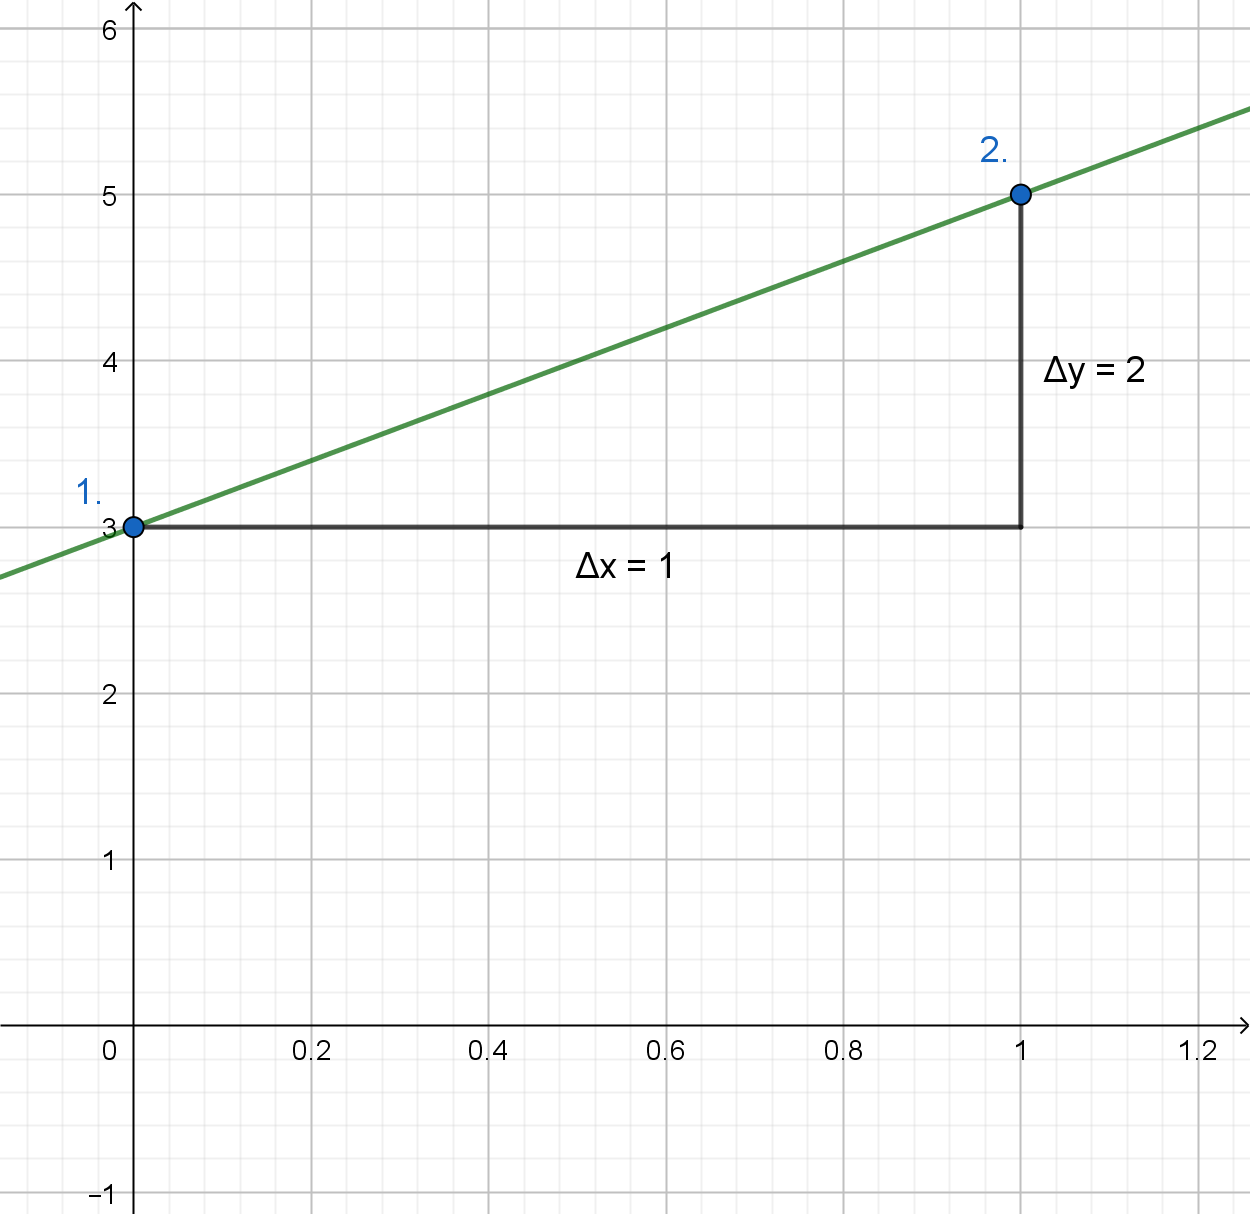
\includegraphics[width=0.48\textwidth]{../99_Bilder/FzG1.png}\\
		\paragraph{(2)} Ist hingegen ein Punkt, z.B. \(P(-1|2)\), und eine Steigung \(m=-\frac{2}{3} (=\frac{\Delta{}y}{\Delta{}x})\) gegeben, übertragen wir zunächst den Punkt in das Koordinatensystem.\\
		Im Anschluss bewegen wir uns \textit{3 Einheiten (\(\Delta{}x\))} nach rechts und dann \textit{2 Einheiten (\(\Delta{}y\))} nach unten (Vorzeichen \(-\)). So gelangen wir zu einem zweiten Punkt \(Q(2|0)\). Die Gerade durch P und Q ist der Graph der Funktion.\\
		\par\noindent
		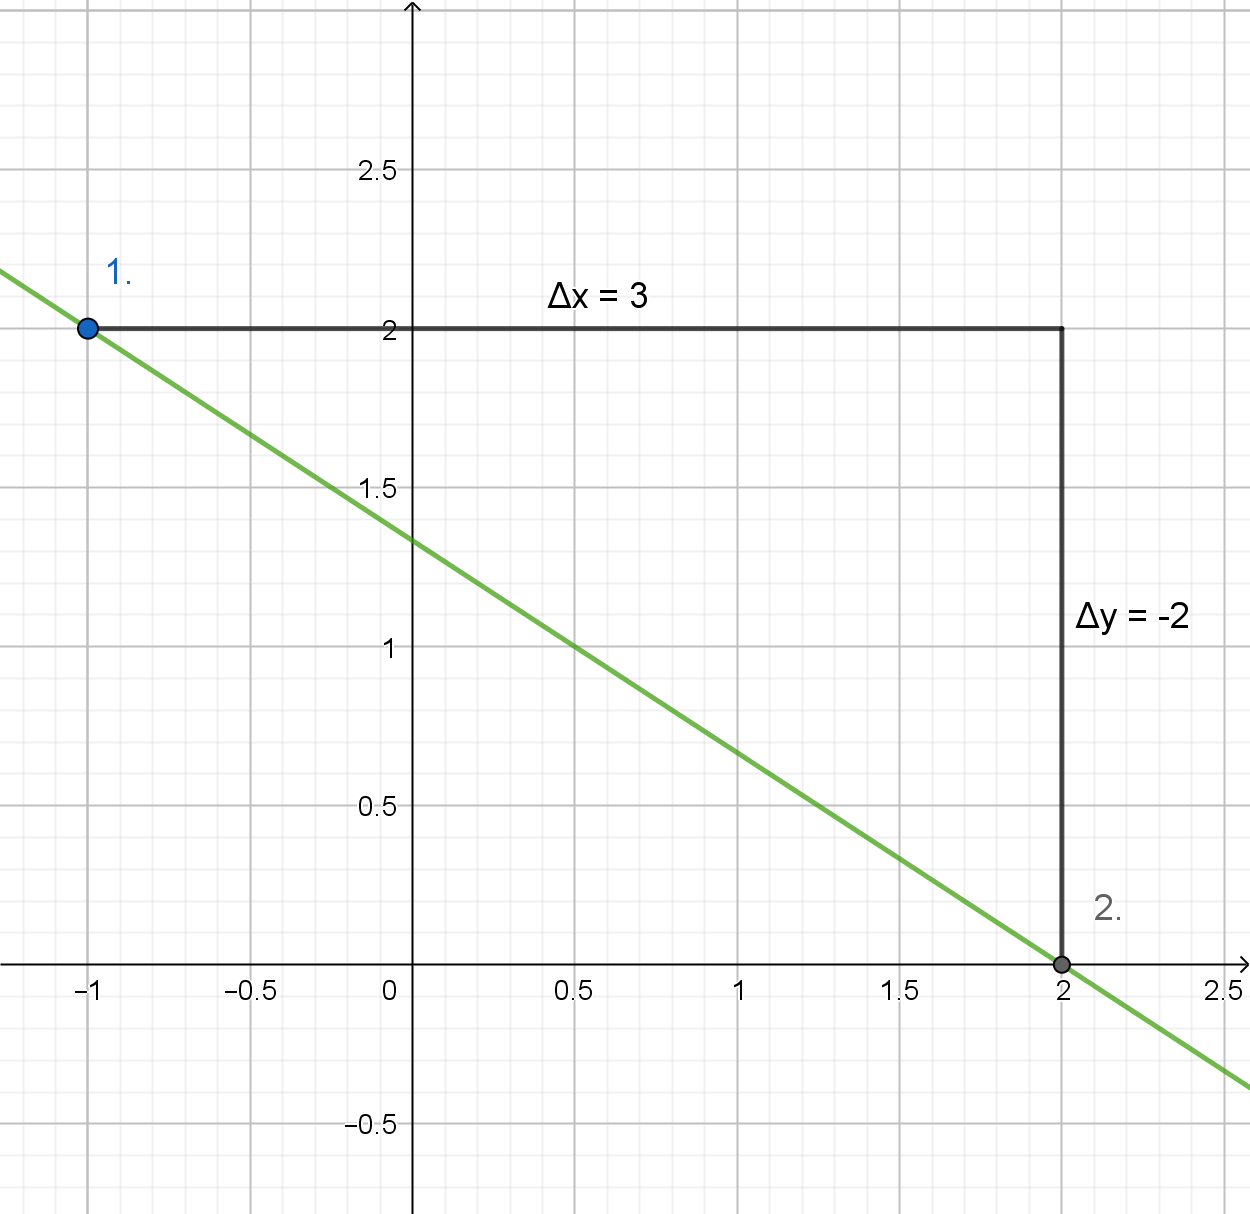
\includegraphics[width=0.48\textwidth]{../99_Bilder/FzG2.png}
		\subsection{Von der Geraden zur Gleichung}
		Aus dem Graphen können wir den Wert für \(b\) direkt ablesen (der Wert, an dem der Graph die y-Achse schneidet).\\
		Um die Steigung zu bestimmen, müssen wir ein Steigungsdreieck einzeichnen und darauf den Quotienten bzw. das Verhältnis der zwei eingezeichneten Seiten bestimmen (\(m = \frac{\Delta{}y}{\Delta{}x}\)).\\
		\par\noindent
		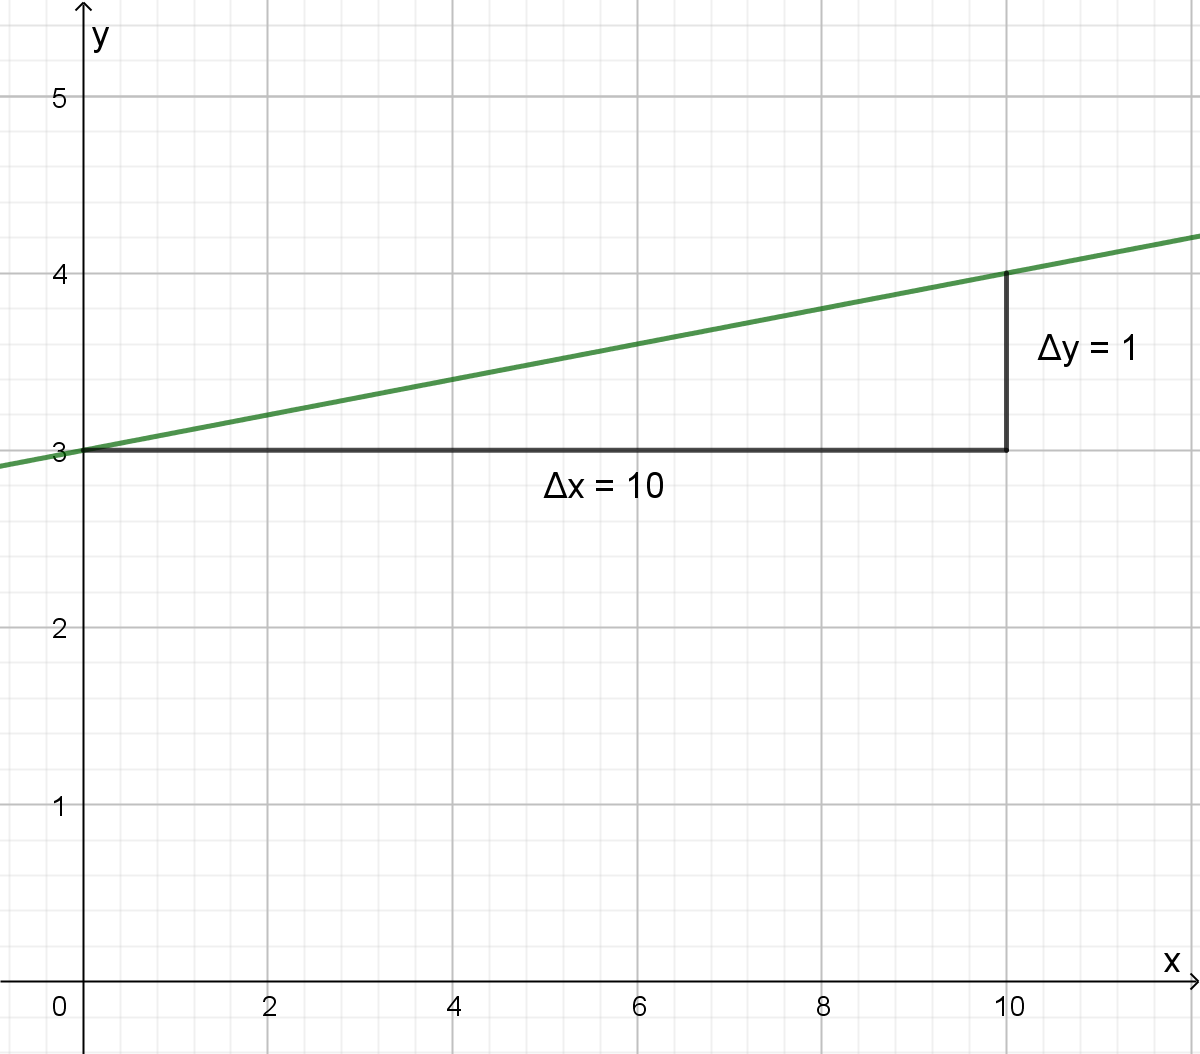
\includegraphics[width=0.48\textwidth]{../99_Bilder/GzF.png}\\
		\par\noindent
		Daraus ergibt sich \(m = \frac{\Delta{}y}{\Delta{}x} = \frac{1}{10}\).\\
		Für die Funktionsgleichung folgt dann
		\[y = \frac{1}{10}x + 3\]
		\subsection{Eine Gerade durch zwei Punkte}
		Haben wir zwei Punkte (z.B. \(P(\underbrace{3}_{x_1}|\underbrace{4}_{y_1})\) und \(Q(\underbrace{7}_{x_2}|\underbrace{6}_{y_2})\)) gegeben, können wir daraus die Funktionsgleichung aufstellen, ohne zeichnen zu müssen.\\
		Wir wissen, dass sich die Steigung als Verhältnis von \(\Delta{}x\) und \(\Delta{}y\) bestimmen lässt (\(m = \frac{\Delta{}y}{\Delta{}x}\)).\\
		Wir berechnen also:\\
		\(\Delta{}x = x_2-x_1 = 7-3 = 4\)\\
		\(\Delta{}y = y_2-y_1 = 6-4 = 2\)\\
		\par\noindent
		Für die Steigung ergibt sich: \(m =\frac{2}{4} = \frac{1}{2}\)
		Anschließend müssen wir den y-Achsenabschnitt bestimmen. Hierfür setzen wir die Koordinaten eines Punktes sowie die berechnete Steigung in die allgemeine Form \(y = mx +b\) ein, und bestimmen den Wert für \(b\).\\
		\par\noindent
		\begin{tabularx}{0.48\textwidth}{ll}
			\(6 = \frac{1}{2}\cdot{}7 + b\) & |\(-\frac{1}{2}\cdot{}7\)\\
			\(2,5 = b\)
		\end{tabularx}\\
		\par\noindent
		Damit haben wir die Funktion bestimmt:
		\[y = \frac{1}{2}\cdot{}x + 2,5\]
		\subsection{Eine Gerade durch einen Punkt mit vorgegebener Steigung}
		Hat man einen Punkt \(P(x_p|y_p)\) und eine Steigung \(m\) gegeben, so lässt sich die Funktionsgleichung direkt mit der Punkt-Steigungsformel aufstellen: \(\mathbf{y=m\cdot{}(x-x_p) + y_p}\).\\
		\subsection{Die Geradengleichung in impliziter Form}
		Bekannt ist uns bereits die lineare Funktion der Form \(y=m\cdot{}x +b\). Nicht immer ist die Funktion in dieser Form gegeben.\\
		Betrachten wir das folgende \textbf{Beispiel}: Eine große Fitness-Studio-Kette möchte eine neue Filiale in Mainz eröffnen. In dieser Filiale sollen zum einen Personal-Trainer beschäftigt werden, die sich auch um die Trainingspläne der Mitglieder kümmern. Zum anderen benötigt man aber auch Service-Personal, dass sich um das Drum-Herum kümmert.\\
		Die Personal-Trainer werden mit \(16.000\) \euro{} und das Service-Personal mit \(4.000\) \euro{}
		äüöplhjm nvcx vergütet. Insgesamt hat sich die Fitness-Kette eine Personalbudget von \(240.000\) \euro{} gesetzt.\\
		Um ein Optimum zu erreichen, sollen alle möglichen Kombinationen der Personal-Trainer und Service-Personal sowohl in einem Graph als auch als Funktionsgleichung dargestellt werden.\\
		\par\noindent
		\begin{tabularx}{0.48\textwidth}{ll}
			\(240.000 = 16.000x + 4.000y\) & |\(-16.000x\)\\
			\(4.000y = -16.000x + 240.000\) & |\(:4.000\)\\
			\(y = -4x + 6.000\) & \(\rightarrow\) Graph
		\end{tabularx}
		\newpage
		\section{Schnittpunkt zweier Geraden}
		Unter bestimmten Umständen kann es notwendig sein, den Schnittpunkt zweier Gerade zu bestimmen. Zum Beispiel, wenn wir zwei Handy-Tarife vergleichen und wissen wollen, ab welcher Anzahl verbrauchter Einheiten (Gesprächsminuten oder SMS) sich der Tarif mit dem höheren Grundpreis lohnt.\\
		\par\noindent
		Das Vorgehen erkunden wir beispielhaft mit Hilfe von \(y_f=2x+1\) und \(y_g = -4x+10\).\\
		\par\noindent
		Es ist möglich, die \textbf{Lösung zeichnerisch} zu bestimmen.\\
		\begin{tabularx}{0.5\textwidth}{XX}
			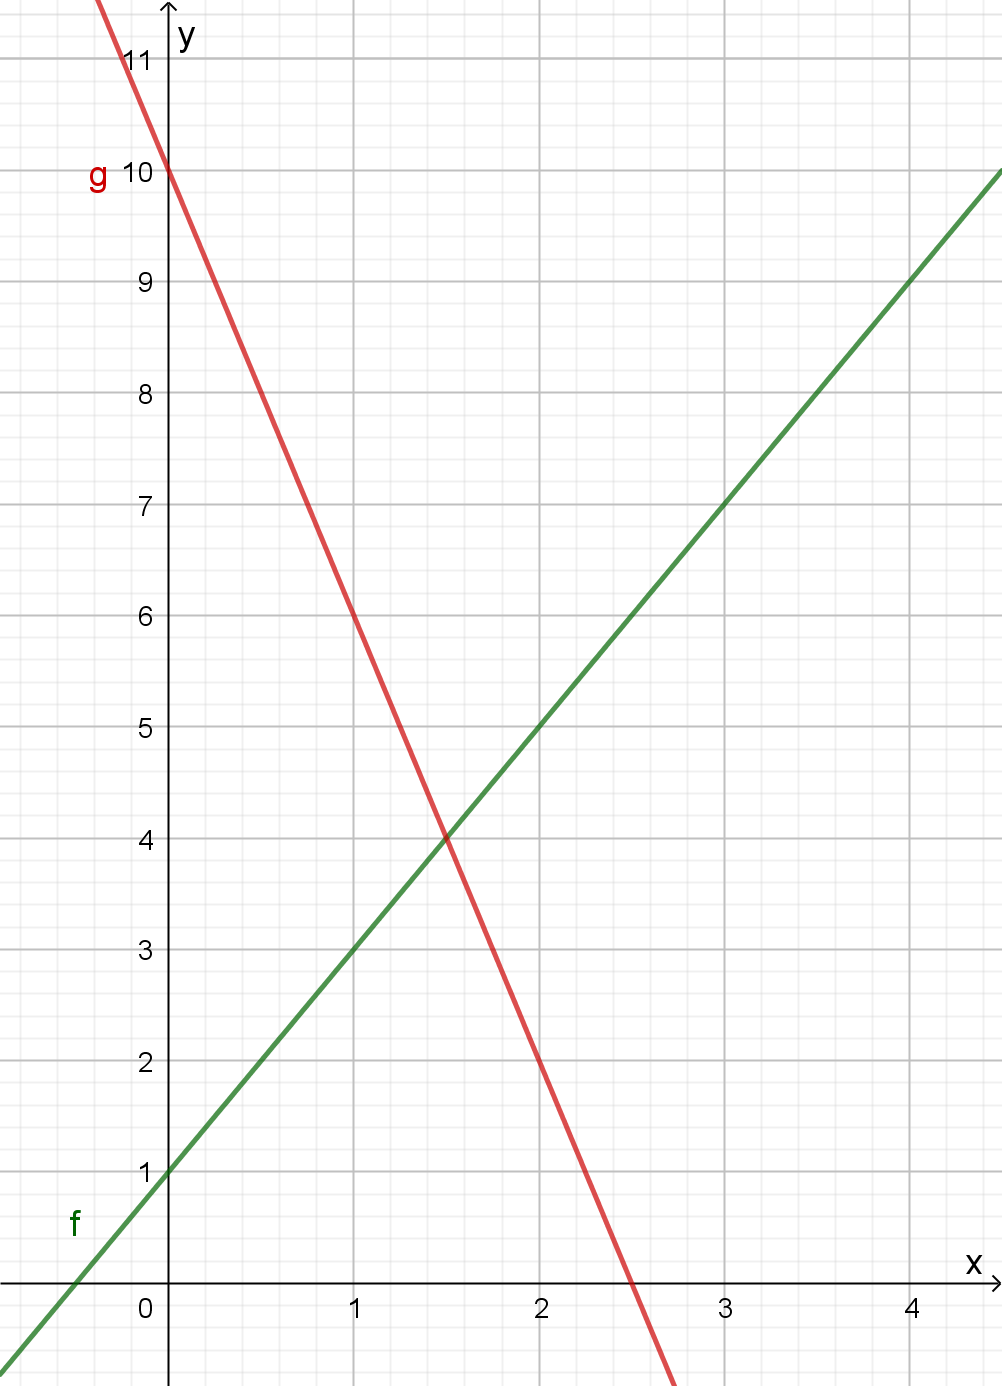
\includegraphics[width=0.24\textwidth,align=t]{../99_Bilder/SzG.png} & \begin{framed}
				Koordinaten des Schnittpunkts: \(SP(1,5|4)\)
			\end{framed}
		\end{tabularx}\\
		\par\noindent
		Um die \textbf{Lösung rechnerisch} zu bestimmen, setzen wir die Funktionen gleich und ermitteln die Lösung für \(x\).\\
		\par\noindent
		\begin{tabularx}{0.48\textwidth}{ll}
			\(2x+1 = -4x+10\) & |\(+4x\)\\
			\(6x + 1 = 10\) & |\(-1\)\\
			\(6x = 9\) & |\(:6\)\\
			\(x = 1,5\)
		\end{tabularx}\\
		\par\noindent
		Wir benötigen nun noch die passende y-Koordinate. \(2\cdot{}1,5 + 1 = 4\).\\
		Also \(SP(1,5|4)\).
		\newpage
		\section{Modellieren mit linearen Funktionen}
		Wie bereits zu Beginn zuvor erwähnt, werden lineare Funktionen verwendet, um Entwicklung mit gleichmäßiger Veränderung widerzuspiegeln.\\
		\par\noindent
		Betrachten wir das Fahrrad-Verleihsystem \glqq{}MVG Mein Rad\grqq{}. Dieses bietet mehrere Tarife, darunter auch\\
		\underline{Normaltarif}: Keine Grundgebühr, \(1,45\) \euro{} pro halbe Stunde\\
		\underline{Tarif Silber}: \(25\) \euro{} Grundgebühr, \(0,85\) \euro{} pro halbe Stunde\\
		\tiny{Quelle: \url{https://www.mainzer-mobilitaet.de/tickets-tarife/fuer-radfahrer/details/tarif/mvgmeinrad-mietradeln-fuer-freibewegliche.html}}\\
		\normalsize
		\par\noindent
		\textbf{Fragestellung}:
		\begin{itemize}
			\item[(a)] Was kosten 50 Stunden in den einzelnen Tarifen?
			\item[(b)] Wann ist der eine Tarif günstiger als der andere?
			\item[(c)] Sie überlegen sich ein Fahrrad für knapp \(120\) \euro{} kaufen. Wie lange könnten Sie für das Geld mit dem \textit{Tarif Silber} fahren?
		\end{itemize}
		\subsection{Der Modellierungsprozess}
		\subsubsection{Aufstellen des Modells}
		Zunächst müssen wir die Preise der jeweiligen Tarife mit Variablen belegen, hierzu wählen wir \(y_N\) für den Normaltarif und \(y_S\) für den Tarif Silber.\\
		Die Kosten beider Tarife sind abhängig von der Dauer, die ein Fahrrad geliehen wird, wobei immer eine halbe Stunde abgerechnet wird. Daher integrieren wir die Variable \(x\) für diese halbe Stunde Ausleihzeit.\\
		Nun ist es uns möglich anhand der Tarifauskunft eine lineare Funktion aufzustellen.\\
		\(y_N = 1,45\cdot{}x\)\\
		\(y_S = 0,85\cdot{}x + 25\)\\
		\subsubsection{Mit dem Modell arbeiten}
		Wollen wir nun schauen, wie wir das Modell nutzen können, um die Fragestellungen zu beantworten.\\
		(a) Wir haben die Ausleihzeit für eine halbe Stunde mit \(x\) modelliert und sollen nun die Kosten nach 50 Stunden berechnen. Daher setzen wir für \(x = 2\cdot{}50 = 100\) ein - eine Stunde \(\widehat{=}\) zwei halbe Stunden.\\
		\(y_N = 1,45\cdot{}100 = 145\)\\
		\(y_S = 0,85\cdot{}100 + 25 = 85+25 = 110\)\\
		\par\noindent
		Antwort: \rule{0.36\textwidth}{0.1pt}\\
		\par\bigskip\noindent
		\rule{0.45\textwidth}{0.1pt}\\
		\par\bigskip\noindent
		\rule{0.45\textwidth}{0.1pt}\\
		\par\noindent
		(b) Übersetzung in das Modell: \(y_N = y_S\).\\
		Wir ersetzen nun \(y_N\) bzw. \(y_S\) durch die Funktionsterme.\\
		\begin{tabularx}{0.5\textwidth}{ll}
			\(1,45\cdot{}x = 0,85\cdot{}x + 25\) & |\(-0,85\cdot{}x\)\\
			\(0,6\cdot{}x = 25\) & |\(:0,6\)\\
			\(x = 41,6\)
		\end{tabularx}\\
		\par\noindent
		Antwort: \rule{0.36\textwidth}{0.1pt}\\
		\par\bigskip\noindent
		\rule{0.45\textwidth}{0.1pt}\\
		\par\bigskip\noindent
		\rule{0.45\textwidth}{0.1pt}\\
		\par\noindent
		(c) Übersetzung in das Modell: \(120 = y_S\).\\
		\begin{tabularx}{0.5\textwidth}{ll}
			\(120 = 0,85\cdot{}x + 25\) & |\(-25\)\\
			\(95 = 0,85\cdot{}x\) & |\(:0,85\)\\
			\(x = 111,76\)
		\end{tabularx}\\
		\par\noindent
		Antwort: \rule{0.36\textwidth}{0.1pt}\\
		\par\bigskip\noindent
		\rule{0.45\textwidth}{0.1pt}\\
		\par\bigskip\noindent
		\rule{0.45\textwidth}{0.1pt}\\
		\par\noindent
	\end{worksheet}
\end{document}